
\pagebreak
\section{Nonlinear equations}
Linear equations can be represented by a matrix. On the other hand, nonlinear equations can't.
Nonlinear equations are about finding roots. They appear in many applications.

\begin{example}
    If we want to solve
    \[ x^2 + 3x + 7 = \log(x) \]
    If we bring it all to one side, then we have to find the root of a function.
    \[ x^2 + 3x + 7 - \log(x) = 0 \]
    Unfortunately, non-linear equations are difficult to solve analytically.
    We can usually approximate the solution by using iterative methods.
\end{example}

\subsection{Bisection method}
\begin{theorem}
    Let $f \in C([a, b])$ ($f(x)$ is continuous on $[a, b]$)
    with $f(a) \cdot f(b) < 0$ (i.e. $f$ has different signs on its ends).
    Then, by continuity, there exists $r \in (a, b)$, such that
    $f(r) = 0$.
\end{theorem}
\begin{remark}
    Actually, this theorem tells that any point between $f(a)$ and $f(b)$ will be achieved.
\end{remark}

\textbf{Idea of the bisection method:}
\begin{enumerate}
    \item {
        Bisection of $[a, b]$ into $[a, c] \cup [c, b]$, i.e.
        into two subintervals, $a < c < b$.
    }
    \item {
        If $f(c) = 0$, then $r = c$, we have found the solution.
    }
    \item {
        If $f(c) \cdot f(a) < 0$, then continue with $[a, c]$.
    }
    \item {
        If $f(c) \cdot f(b) < 0$, continue with $[c, b]$.
    }
\end{enumerate}
\begin{remark}
    When $f(a) \cdot f(b) > 0$, $f$ may or may not have a root on $[a, b]$ ---
    we cannot say for sure.
\end{remark}
\begin{remark}
    This algorithm will only find one root, not all.
\end{remark}

\textbf{The method in short:}

Producing a sequence of intervals $[a_i, b_i]$ such that a root $r$ is inside these intervals.
The starting interval is $[a, b] = [a_0, b_0]$.

\begin{theorem}
    The bisection method, when applied to $[a, b]$ and 
    $f \in C^*([a, b])$ with $f(a) \cdot f(b) < 0$ will complete after
    $n$ steps an approximation $c_n$ of root $r$ with error
    \[ \abs{r - c_n} < \frac{b - a}{2^n} \]
\end{theorem}
\begin{remark}
    If we do infinitely many iterations, we will always find the root, because
    \[ \lim_{n \to \infty} \frac{b - a}{2^n} = 0 \]
\end{remark}
\begin{proof}
    At every step, the length of the interval where the root is located
    is divided into two. We can use induction to prove the above-mentioned error formula.
\end{proof}

\begin{example}
    Let $[a, b] = [0, 1]$. How many iterations are needed to decrease the error
    below $2^{-20} \approx 10^{-6}$?

    We need to find an $n \in \mathbb{N}$, such that our error estimate
    is less than what we want:
    \begin{align*}
        &
        \frac{b - a}{2^n} < 2^{-20} \Longleftrightarrow
        \frac{b - a}{2^{-20}} < 2^n \Longleftrightarrow
        \log_2\Bigl(\frac{b - a}{2^{-20}}\Bigr) 
        \overset{\text{$\log_2$ is strictly increasing}}{<} \log(2^n) = n
        \\&
        \log_2\Bigl(\frac{1}{2^{-20}}\Bigr) < n \Longleftrightarrow
        \log_{2}(1) - \log_{2}(2^{-20}) < n \Longleftrightarrow
        0 - (-20) < n \Longleftrightarrow 20 < n
    \end{align*}
\end{example}
\begin{remark}
    The bisection method has a slow convergence.
    For every iteration step we get a \textit{binary} digit as our accuracy increase.
    Recall that for approximating $\cos(x)$ by Taylor polynomial,
    we get 2 decimal digits per term of the polynomial. 
\end{remark}

\subsection{Newton method}

\begin{definition}
    Suppose that the sequence $\{x_n\}$ converges as $n \to \infty$.
    Then the sequence:
    \begin{enumerate}[label=\alph*)]
        \item {
            converges \textit{linearly} to $r$, if 
            there exists such an $M \in (0, 1)$, such that
            \[ \lim_{n \to \infty} \frac{\abs{x_{n + 1} - r}}{\abs{x_{n} - r}} = M \]
            \begin{example}
                For bisection method $M = \frac{1}{2}$.
            \end{example}
        }
        \item {
            converges \textit{super-linearly} to $r$, if
            \[ \lim_{n \to \infty} \frac{\abs{x_{n + 1} - r}}{\abs{x_{n} - r}} = 0 \]
        }
        \item {
            converges \textit{sub-linearly} to $r$, if
            \[ \lim_{n \to \infty} \frac{\abs{x_{n + 1} - r}}{\abs{x_{n} - r}} = 1 \]
            (i.e. at some point the error decrease rate stagnates).
        }
        \item {
            converges \textit{with order $q > 1$}, if there exists $M > 0$, such that
            \[ \lim_{n \to \infty} \frac{\abs{x_{n + 1} - r}}{\abs{x_{n} - r}^q} < M \]
            If $q = 2$, the convergence is called \textit{quadratic},
            if $q = 3$ --- cubic.
        }
    \end{enumerate}
\end{definition}

\begin{definition}[Newton method]
    Let $f \in C^1([a, b])$. Then at every 
    $x_0 \in (a, b)$ there exists a tangent to the graph of $f$.
    The tangent equation at $x_0$ can be written as follows:
    \begin{align*}
        &
        t(x) = f(x_0) + f'(x_0)(x - x_0)
        \\&
        \frac{t(x) - f(x_0)}{x - x_0} = f'(x_0)
    \end{align*}
    If we recall, the tangent at $x_0$ is the first order Taylor polynomial of $f(x)$
    with $t(x_0) = f(x_0),\ t'(x) = f'(x_0)$.
    \pagebreak
    \begin{figure*}[h]
        \centering
        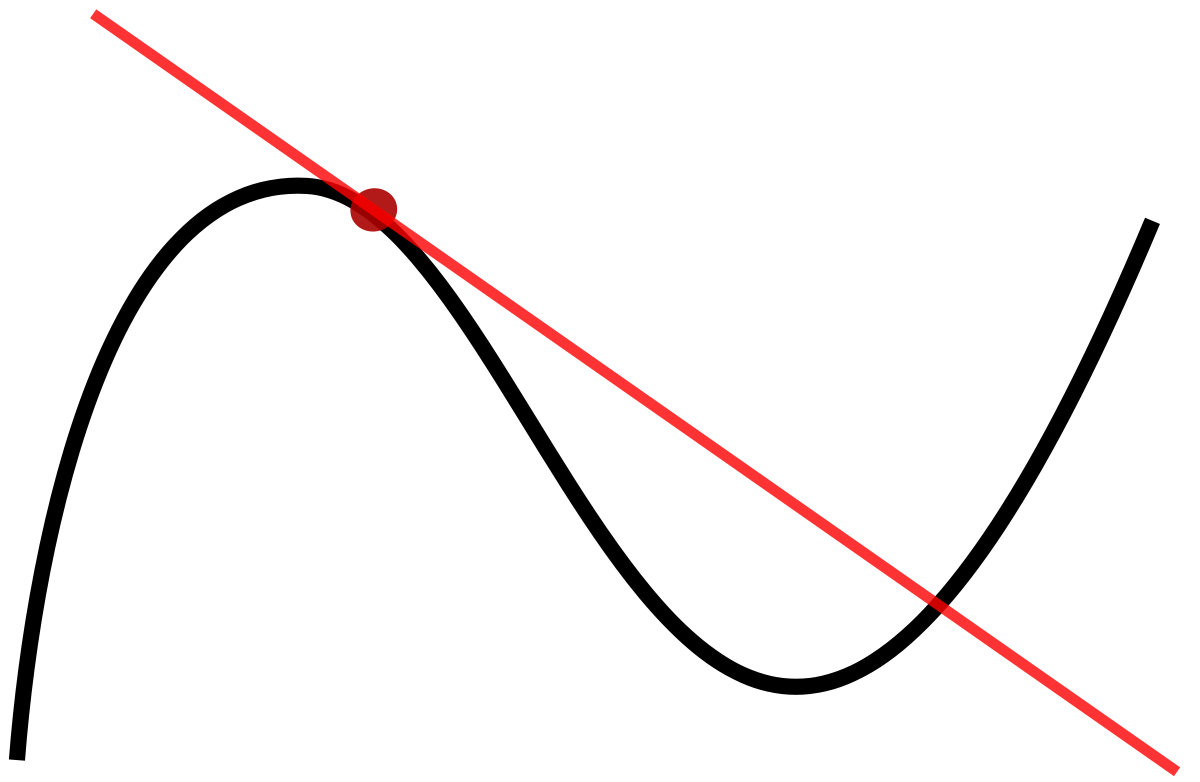
\includegraphics[width=0.3\textwidth]{tangent}
    \end{figure*}

    We use the tangent $t(x)$ as an approximation to $f(x)$,
    and we can find the root of $t(x)$ easily, as it's a linear funciton:
    \[
        0 = t(x_1) = f(x_0) + f'(x_0)(x_1 - x_0) \Longleftrightarrow
        x_1 = x_0 - \frac{f(x_0)}{f'(x_0)}
    \]

    Continuing yields the Newton sequence (Newton–Raphson iteration):
    \[ x_{n + 1} = x_n - \frac{f(x_n)}{f'(x_n)},\ x_0 = \text{initial guess} \]

    \begin{figure*}[h]
        \centering
        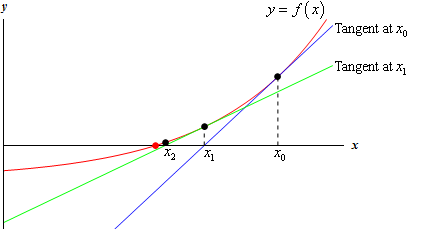
\includegraphics[width=0.5\textwidth]{newton}
    \end{figure*}

    Here we cannot have $f'(x_n) = 0$, since we cannot divide by zero. Therefore,
    it's often a good idea to make sure $f'$ doesn't have roots on the interval
    of search.
\end{definition}
%\begin{theorem}
%    When the Newton sequence converges, it converges to
%    \textbf{a} root of $f$.
%\end{theorem}